Maskinens degform ska stänga Raviolidegen med hjälp av två likströmsmotorer. Motorers rotationsenergi ska överföras till degformen med användning av kugghjulsväxel.  Genom avläsning av motorers ström kan man upptäcka när formen har pressat Raviolidegen tillräcklig mycket.\\

Det är också tänkt att implementera möjligheten att hissa upp och ner maskinens degform. Detta görs för att minska avstånd mellan maskinens degform och pump. För att genomföra detta ska en kuggväxel bestående av två kugghjul och två kuggsträngar användas, se figur.~\ref{maskinens_baksida_metod}

\begin{figure}[ht]
	\begin{center}
		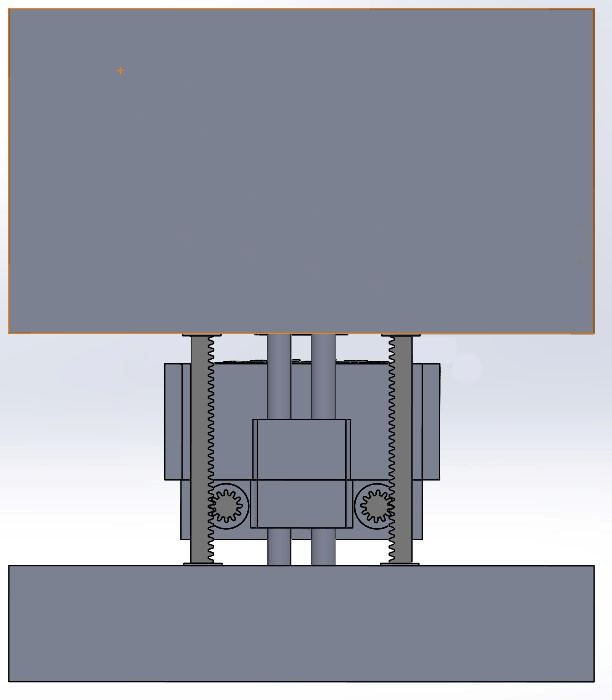
\includegraphics[scale=0.8]{images/maskinenshiss.jpg}
		\caption{Maskinens baksida som innehåller kuggsträngar och kugghjul(kuggväxel)}
		\label{maskinens_baksida_metod}	
	\end{center}
\end{figure}
